\section{Smart Homes \& Smart Hubs}\label{sec:smarthomes}
Smart homes is, as mentioned, also a trending concept. 
Berg Insight have compiled a report \cite{SMARTHOMETREND}, 
showing that the number of smart homes in North America and in Europe is rising steadily. 
They have illustrated this as a bar chart, reproduced in \Cref{fig:smarthomestrend}.
They define a smart home as having a \emph{smart home system}, 
but do not further define what such a system is, 
but we can conclude that the homes have at least one smart device each. 

\begin{figure}[!htb]
  \centering
  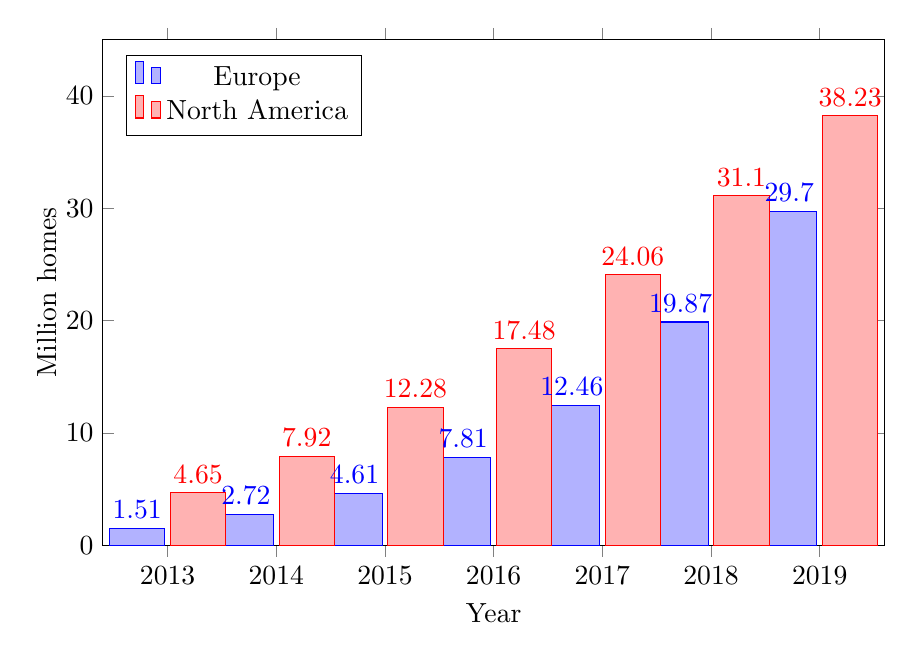
\begin{tikzpicture}
    \begin{axis}[
        height=8cm,
        width=0.95\textwidth,
        xlabel={Year},
        ylabel={Million homes},
        yticklabel style={align=right,inner sep=0pt,xshift=-0.3em},
        scaled y ticks = false,
        nodes near coords align={vertical},
        nodes near coords,
        xtick=data,
        symbolic x coords={2013, 2014, 2015, 2016, 2017, 2018, 2019},
        ybar,
        ymax=45,
        ymin=0,
        bar width=20pt,
        legend pos = north west,
        ]
        \addplot coordinates {(2013, 1.51) (2014, 2.72) (2015, 4.61) (2016, 7.81) (2017, 12.46) (2018, 19.87) (2019, 29.70)};        
        \addplot coordinates {(2013, 4.65) (2014, 7.92) (2015, 12.28) (2016, 17.48) (2017, 24.06) (2018, 31.10) (2019, 38.23)};
        \legend{Europe, North America}
        
        %Trend lines:
%        \addplot [ultra thick,orange,line join=round,smooth, nodes near coords = ] coordinates {(2013, 1.51) (2014, 2.72) (2015, 4.61) (2016, 7.81) (2017, 12.46) (2018, 19.87) (2019, 29.70)};
%        \addplot [ultra thick,orange,line join=round,smooth, nodes near coords = ] coordinates {(2013, 4.65) (2014, 7.92) (2015, 12.28) (2016, 17.48) (2017, 24.06) (2018, 31.10) (2019, 38.23)};
%        

    \end{axis}
\end{tikzpicture}
  \caption{Smart homes trend based on sales and statistics. Data from \protect\cite{SMARTHOMETREND}.}
  \label{fig:smarthomestrend}
\end{figure}

The elements in smart homes can be categorized into:
\begin{enumerate}
  \item Sensors - Capable of observing the environment
  \item Actuators - Control parts of the environment (\eg lights or air condition units)
  \item Software Clients - Controls the actuators based on input from the sensors
\end{enumerate}

We will not discuss the sensors of smart homes much in this report, 
but will rather talk about the \emph{actuators}, 
\ie the controllable smart devices,
and the software clients that control the actuators in a smart home.

The devices found in smart homes are common items, 
that have been connected to the Internet for wireless control.
Common devices that are found in smart homes include, but are not limited to, 
windows, HVAC (heating, ventilating, and air conditioning) units, thermostats, sound systems and locks. 

However, only few devices have really gained ground for the common user and few homes are automated.
A smart device that is currently becoming more popular is the Nest thermostat \footnote{\url{https://nest.com/}}. 

This thermostat senses when you are around, and when you are not, 
to control the climate inside to save energy and thus money.
Unlike a lot of smart devices that are made to make your life a little easier, such as smart bulbs or HVAC units,
the Nest thermostat helps you save money which is likely the reason for it popularity. 
Furthermore, the newest version (as of October 2015) allows you to connect other smart devices to the thermostat, 
using the Weave protocol. 
The Nest thermostat is thus starting to solve what is likely the greatest problem with smart homes and IoT in general, 
and why they have not become popular yet: lack of interoperability between smart devices. 
The Nest thermostat is, however, limited in this, 
as it only supports the Weave protocol. 

\Cref{table:iotprotocols} shows \emph{some} of the many different protocols, 
that are being used by smart devices. 
The Nest thermostat is able to communicate with the other devices that uses the Weave protocol, 
but it cannot communicate with other devices that uses \eg the ZigBee or Z-Wave protocol. 

\begin{table}[!htb]
  \begin{description}
    \item[Protocol:] ZigBee
    \item[Used by:] Samsung, Jasco, Smartenit, FortrezZ and others
    \item[In products:] SmartThings Hub, thermostats, door sensors, light bulbs, etc.\\
    
    \item[Protocol:] Z-Wave
    \item[Used by:] FortrezZ, GE, Intermatic, Leviton, Aeon Labs, Evolve and others
    \item[In products:] Thermostats, wall outlets, door locks, door and window sensors, etc.  \\
    
    \item[Protocol:] WiFi (IEEE 802.11)
    \item[Used by:] Nest, Philips, Samsung, Bose, D-link and others
    \item[In products:] Thermostats, speakers, light bulbs, motion sensors, fitness trackers, camera, etc. \\
    
    \item[Protocol:] Weave
    \item[Used by:] Nest, Philips, pebble, Logitech, Jawbone and others
    \item[In products:] Thermostats, fitness trackers, camera, lights, locks, etc. 
  \end{description}
  \caption{Wireless protocols used by smart devices}\label{table:iotprotocols}
\end{table}

Researchers and companies are working on developing what we call \emph{smart hubs}. 
A smart hub is a device, or service, 
that implements several communication protocols used by IoT devices, 
and gives the user a single protocol or interface. 
The goal of a smart hub is to enable the connected devices to communicate.
The communication problem arises from the number of different communication protocols used by the smart devices. 
In the following section we will analyze a smart hub called HomePort. 

\subsection{Analysis of a Smart Hub: HomePort}\label{sec:homeport}
In this section we will analyze a smart hub called \emph{HomePort} \cite{HOMEPORT10}.
HomePort is not a commercial smart hub, 
but is a research project at the Institute of Computer Science, Aalborg University in Denmark. 
The reason why we are analyzing this smart hub, 
is that it is described in a way that commercial smart hubs are not (either due to secrecy or simply lack of information) \cite{HOMEPORT09, HOMEPORT10, HOMEPORT13}.  

HomePort is technically a system, or rather an architecture, rather than a hub. 
The architecture is described in \cite{HOMEPORT10}. 
However, an implementation of this, \ie an actual smart hub, can be found in \cite{HOMEPORT13}. 
The architecture consists of \num{4} layers as illustrated by \Cref{fig:homeport}.

\begin{figure}[!htb]
    \centering
    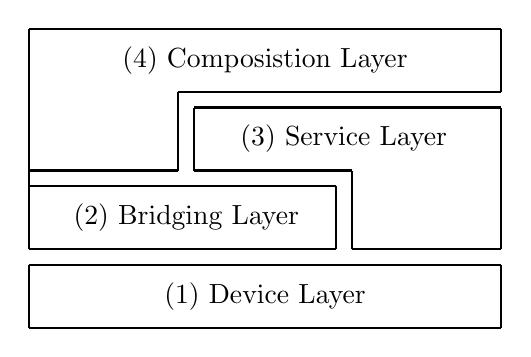
\begin{tikzpicture}
    \node at (0, 2) {(4) Composistion Layer};
    \node at (1, 1) {(3) Service Layer};
    \node at (-1, 0) {(2) Bridging Layer};
    \node at (0, -1) {(1) Device Layer};
    
    %Composition Layer Box
    \draw[thick,-] (3,2.4) -- (-3,2.4);
    \draw[thick,-] (-3,2.4) -- (-3,0.6);
    \draw[thick,-] (3,2.4) -- (3,1.6);
    \draw[thick,-] (-3,0.6) -- (-1.1,0.6);
    \draw[thick,-] (3,1.6) -- (-1.1,1.6);
    \draw[thick,-] (-1.1,0.6) -- (-1.1,1.6);
    
    %Service Layer Box
    \draw[thick,-] (3,1.4) -- (-0.9,1.4);
    \draw[thick,-] (3,1.4) -- (3,-0.4);
    \draw[thick,-] (3,-0.4) -- (1.1,-0.4);
    \draw[thick,-] (1.1,-0.4) -- (1.1,0.6);
    \draw[thick,-] (1.1, 0.6) -- (-0.9,0.6);
    \draw[thick,-] (-0.9, 0.6) -- (-0.9,1.4);

    %Bridging Layer Box
    \draw[thick,-] (-3,0.4) -- (0.9, 0.4);
    \draw[thick,-] (0.9, 0.4) -- (0.9, -0.4);
    \draw[thick,-] (0.9, -0.4) -- (-3, -0.4);
    \draw[thick,-] (-3, -0.4) -- (-3, 0.6);
    
    %Bridging Layer Box
    \draw[thick,-] (-3,-0.6) -- (3, -0.6);
    \draw[thick,-] (3, -0.6) -- (3, -1.4);
    \draw[thick,-] (3, -1.4) -- (-3, -1.4);
    \draw[thick,-] (-3, -1.4) -- (-3, -0.6);
\end{tikzpicture}
    \caption{The HomePort architecture proposed in \protect\cite{HOMEPORT10}.}
    \label{fig:homeport}
\end{figure}

The layers have the following functionality:
\begin{description}
    \item[(1) Device Layer] This layer consists of the smart devices connected to each subsystem (\eg ZigBee or Z-wave). Devices in different subsystems can usually not communicate with each other, due to lack of common protocols. 
    \item[(2) Bridging Layer] This layer relays commands from one subsystem to another using minimum translation or adaption of the subsystem protocols. Commands are sent to a \emph{bridge device}, which then replies on behalf of the other devices. The layer consists of two parts: a generic bridging part and a subsystem dependent part. 
    \item[(3) Service Layer] This layer provides the composition layer with device functionality using a common language. A Gateway device is introduced to give access to the Bridge devices. This Gateway device communicates using a RESTful interface. 
    \item[(4) Composition Layer] The composition layer lets applications use multiple home devices to create a smart home, by communicating with the different Bridge devices through the common language from the service layer. 
\end{description}

The implementation of HomePort \cite{HOMEPORT13}, 
modified a few things about this architecture, 
and added additional components such as a logging system. 
An illustration of the implemented system can be seen in \Cref{fig:homeport2}.
The implementation runs on a Linux server and uses ZeroConf to discover services on the network. 
Clients (\eg applications) communicate with the smart devices through HomePort. 
The clients can get a list of devices in the system by sending a GET request, 
which also returns the services they provide. 

\begin{figure}[!htb]
    \centering
    \tikzstyle{block} = [rectangle,draw,minimum width=3cm, minimum height = 1cm, text width=2.7cm]
\tikzstyle{longblock} = [rectangle,draw,minimum width=9cm, text width=8.7cm]
\begin{tikzpicture}[every text node part/.style={align=center}]
\small
\node[rectangle,draw] at (-3, 0) {Client 1};
\node[rectangle,draw] at (0, 0) {Client 2};
\node[rectangle,draw] at (3, 0) {Client n};

\node at (-4.2, -2) {HomePort};

\node[block] at (-3, -3) {Webserver};
\node[block] at (0, -3) {ZeroConf};
\node[block] at (3, -3) {Log};

\node[block] at (-3, -4) {HomePort Services};
\node[block] at (0, -4) {HomePort Secure Services};
\node[block] at (3, -4) {HomePort Access Control Service};

\node[longblock, minimum height=0.5cm] at (0, -4.750) {Events Module};
\node[longblock, minimum height=0.5cm] at (0, -5.275) {Configuration};
\node[longblock, minimum height = 1cm] at (0, -6.05) {Adapter $1, 2, \ldots, n$};

\node[rectangle,draw,minimum width=0.68\textwidth, minimum height=1cm] at (0, -7.05) {OS (Linux)};

\node[rectangle,draw] at (-3, -9) {Device 1};
\node[rectangle,draw] at (-1, -9) {Device 2};
\node[] at (1, -9) {$\ldots$};
\node[rectangle,draw] at (3, -9) {Device n};

\node[rectangle,draw, minimum width=0.7\textwidth, minimum height=6cm] at (0, -4.7) {};

\node[cloud, cloud puffs=20.7, cloud ignores aspect, minimum width=8cm, minimum height=2.5cm, align=center, draw] (cloud) at (0, 0) {};
\draw[triangle 90-triangle 90,line width=0.5mm] (0,-1) -- (0, -1.75);

\draw[triangle 90-triangle 90,line width=0.5mm] (-3,-8.8) -- (-3, -7.7);
\draw[triangle 90-triangle 90,line width=0.5mm] (-1,-8.8) -- (-1, -7.7);
\draw[triangle 90-triangle 90,line width=0.5mm] (3,-8.8) -- (3, -7.7);
\end{tikzpicture}
    \caption{The HomePort architecture implemented in \protect\cite{HOMEPORT13}.}
    \label{fig:homeport2}
\end{figure}

Following is a short description of the HomePort system showed in \Cref{fig:homeport2}:
\begin{description}
    \item[Webserver] Provides a RESTful interface to access and control the services.
    \item[ZeroConf] A service discovery module that discovers devices inside a Local Area Network (LAN).
    \item[Log] The log module keeps trace of requests and events. 
    \item[HomePort Services] Keeps information about the services. 
    \item[HomePort Secure Services] Adds security through TLS to the HTTP requests (HTTPS).
    \item[HomePort Access Control Service] This module contains a table of information about what each client is allowed to do. 
    \item[Events Module] Sends notifications to devices and handles requests from clients.
    \item[Configuration] Stores configuration of HomePort. HomePort can be configured to use only HTTP, a mix of HTTP and HTTPS or only HTTPS.
    \item[Adapter] The adapters handles the translation between devices. 
\end{description}

HomePort uses, as mentioned, a RESTful interface for communication. 
In order to get the devices in the HomePort network, 
we can do a GET request on \texttt{/devices}.
The output is an XML file containing information about the devices,
such as ID and what actions can be performed,
or rather what values the devices can have (\eg 0 = off, and 1 = on).
Each device also has an URL. 
This URL is used to control the devices. 

\FloatBarrier
\subsubsection{Example of HomePort}
Following is an example of how to turn on a lamp in HomePort.
In this example, the lamp is connected to a Phidget\footnote{\url{http://www.phidgets.com/}} network, 
where HomePort is connected to a Phidget interface kit with ID \texttt{173111}, 
using a Phidget adapter. 
We have borrowed a box (\Cref{fig:phidget-box}) with a Phidget interface kit and two light bulbs (simulating lamps) from Aalborg University.
We want to change the \emph{output} of the lamp with ID \texttt{0} (the right lamp in \Cref{fig:phidget-box}),
to the value \texttt{1}, \ie turn the lamp on. 
To change the value of the lamp, 
we must send the following XML data to it:

\begin{minted}[autogobble]{xml}
  <?xml version='1.0' encoding='UTF-8'?><value>1</value>
\end{minted}

\begin{figure}[!htb]
	\centering
	\subbottom[Both lamps off]{\label{fig:phidget-box:off}
	  	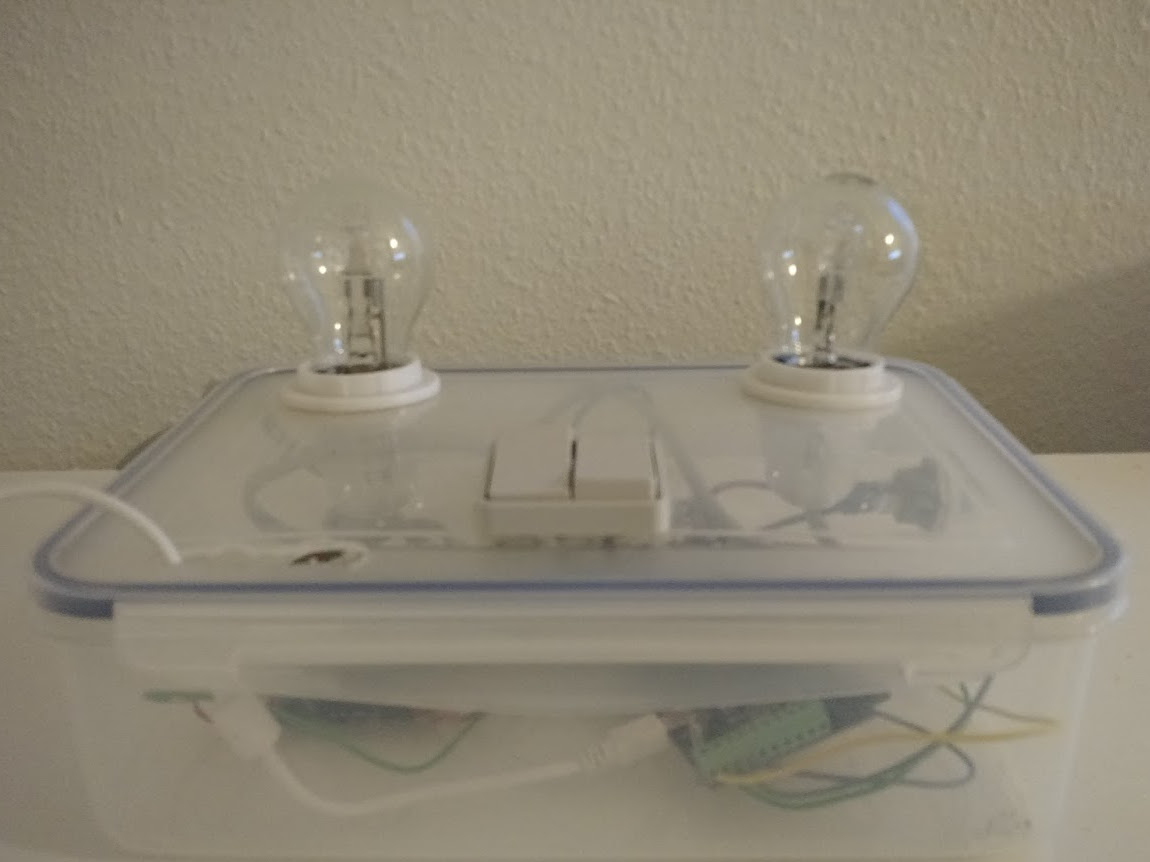
\includegraphics[width=0.45\textwidth]{images/phidget_off}
	}\hfill
	\subbottom[Lamp with ID 0 is on]{\label{fig:phidget-box:on}
	  	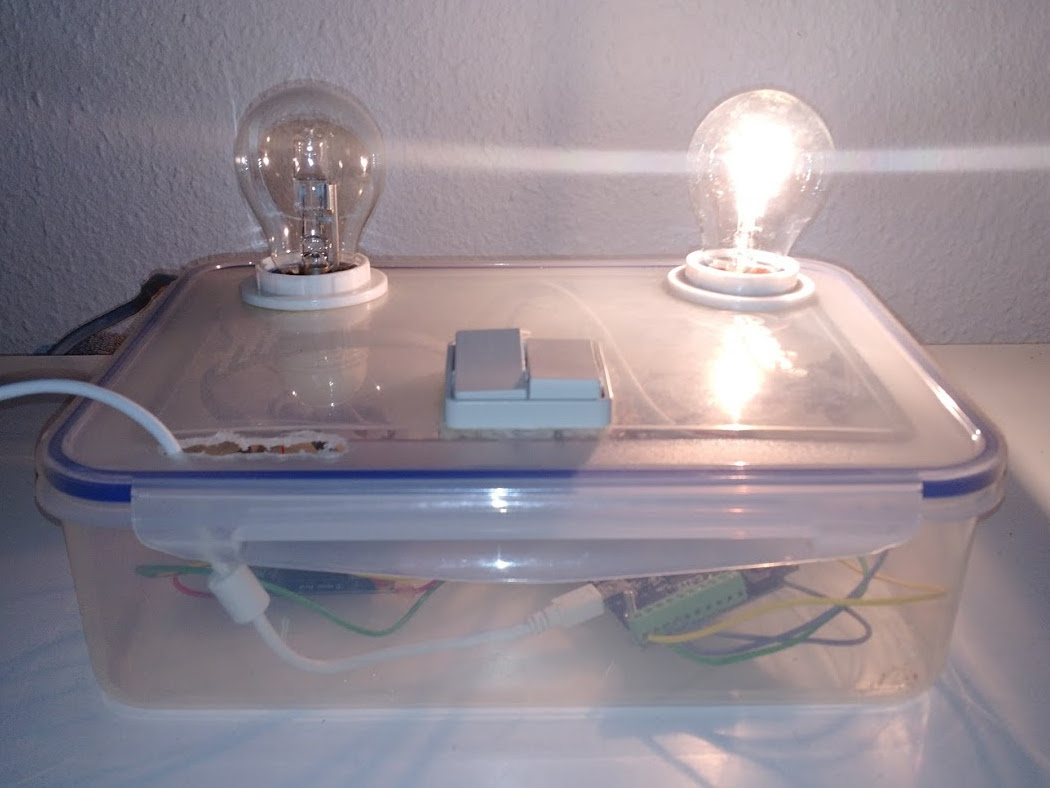
\includegraphics[width=0.45\textwidth]{images/phidget_on}
	}
	\caption{Phidget box with a Phidget interface kit, a relay and two light bulbs connected to HomePort}
	\label{fig:phidget-box}
\end{figure}

The data is sent as a PUT request with the URL of the lamp, 
which in this example is \texttt{/phidget/173111/output/0}. 
The URL describes that we want to change the \texttt{output} of device with ID \texttt{0}, 
of the network interface with ID \texttt{173111}, to the value \texttt{1}.
The result of this PUT request is \Cref{fig:phidget-box:on}.

From what we have seen so far with HomePort, 
it shows that only a part of the smart hub's responsibility, 
is the translation between the different protocols. 
The smart hub should also handle requests from clients (\eg using a RESTful interface), 
and preferably also provide secure communication. 

\subsection{Smart Hubs on the Market}\label{sec:smarthubsmarket}
The requirements for smart hubs have gained the attention of several large companies, 
and even more smaller companies, 
all competing to be the center of future smart homes. 
One of the mature commercial available smart hubs, 
is the Samsung SmartThings Hub \cite{SMARTTHINGS}. 
The SmartThings Hub is a standalone device, 
that supports the Z-Wave, ZigBee and WiFi protocols, 
and provides a smartphone application and a RESTful interface. 
The SmartThings Hub has been tested, 
and is compatible with more than \num{150} devices as of October 2015.
With support for the aforementioned protocols, 
and a REST interface, this number is in practice higher.  
The price for such a hub is \$99, 
which is, compared to the prices for some of the compatible devices, very affordable. 

Samsung is, however, not the only company selling smart hubs. 
Microsoft has been working on their HomeOS \cite{HOMEOS}, 
and Apple has their HomeKit \cite{HOMEKIT}.
While these products differ in terms of architecture, descriptions (operating system contra hub) and availability,
they all share the same goal of giving a centralized control of smart devices. 

There are also other open source alternatives such as openHAB \cite{OPENHAB}, 
where you setup your own server running the open sourced code, 
and control the devices through that. 
The advantage here is of course the price (free), 
and the possibility of adding new unsupported products. 

\Cref{table:smarthubs} gives a short overview of some of the available or coming smart hubs. 
\begin{table}
    \centering
    \begin{tabular}{l l}
        Company                           & Product Type \\ \hline
        openHAB \cite{OPENHAB}            & Employ open source code on own server \\
        Open Source Automation \cite{OSA} & Employ open source code on own server \\
        OpenRemote \cite{OPENREMOTE}      & Employ open source code on own server \\
        Apple \cite{HOMEKIT}              & HomeKit Framework \\
        Samsung \cite{SMARTTHINGS}        & SmartThings Hub: A standalone device that costs \$99 \\
        Microsoft \cite{HOMEOS}           & HomeOS: An operating system that runs on a server
    \end{tabular}
    \caption{An overview of home automation hubs from different companies.}
    \label{table:smarthubs}
\end{table}

\subsection{Control of Smart Homes}\label{sec:smarthomecontrol}
While smart hubs let different smart devices communicate, 
they are not meant to be a control panel for smart homes (although some, such as HomeOS, is designed as such).
To control the devices connected to a smart home, or standalone smart devices, 
most vendors offer a smartphone applications, 
that give the consumer a basic interface to control the device and set rules for it, \etc.
This is for example the case with the Samsung SmartThings Hub. 

An alternative to such a smartphone application, 
could be the Logitech Harmony Remote \cite{HARMONYREMOTE}, 
which is a universal remote that can connect to over \num{270000} devices (smart and dumb). 
It comes either as a standalone remote control or connected with a hub. 
Depending on the model, the remote either uses infrared (does not require a hub), 
or connects to a hub via WiFi. 

Gesture control is a alternative way of controlling a smart home. 
We have already mentioned the HIRIS computer, 
that is able to track 3D movements, and thus 3D gestures, 
but in this section we want to explore another solution that are designed for smart homes. 

A company known as Reemo \cite{Reemo}, formerly Playtabase, 
has created a way of controlling smart devices in homes using gestures. 
They have developed a wearable device which is located on the wrist. 
The wearable allows user to point at a device, 
and then perform a pre-programmed gesture, 
which corresponds to a certain action for that device. 
A small receiver must be placed near the devices that you want to control. 
The receiver must be pointed at as depicted by \Cref{fig:reemo}.
The pointing will, however, only work, 
if the device is line of sight of the wearable. 

\begin{figure}[!htb]
    \centering
    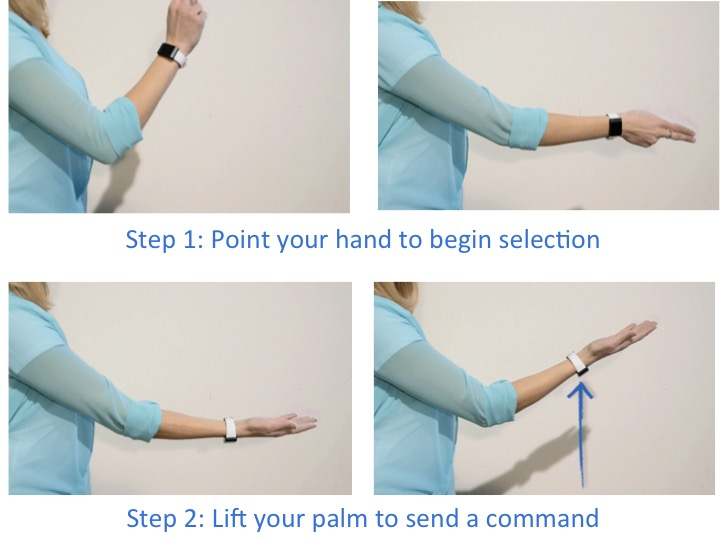
\includegraphics[width=0.8\textwidth]{images/Reemo}
    \caption{How Reemo gesture control works. Source: \url{http://www.getreemo.com/projects/}.}
    \label{fig:reemo}
\end{figure}

Unfortunately they have not disclosed any details regarding the technology, 
how the system knows which receiver you are pointing at, 
or how the devices are controlled. 
The company and the product is also still in a development phase, 
so the product is not commercialized yet, 
but have been in development since mid-2014.

These are the most common and/or most intuitive ways of controlling smart devices. 
The question is which solution is ``the best'', 
or rather, which method is the wanted way of controlling the devices.
\Cref{tbl:smartcontrol} summaries the aforementioned 3 ways. 

\begin{table}[!htb]
    \centering
    \parbox[t][][t]{0.3\textwidth}{
        \textbf{Smartphone Application}\\
        \textbf{Pros:} Easy control of smart devices if the smartphone is usually carried or always near. 
                       Applications are usually available from vendors. 
                       Easy to get updates to the software. \\
        \textbf{Cons:} Requires a smartphone nearby to control. 
                       An overhead of unlocking phone, opening application and selecting device and action.
    }\quad
    \parbox[t][][t]{0.3\textwidth}{
        \textbf{Remote Control}\\
        \textbf{Pros:} Easy control of smart devices if the remote is usually carried or always near. \\
        \textbf{Cons:} Requires a remote control nearby to control (usually not very expensive). 
                       An overhead of selecting device and action.
    }\quad
    \parbox[t][][t]{0.3\textwidth}{
        \textbf{Gesture Control}\\
        \textbf{Pros:} Wearables are usually worn and grants easy control of applications by gesture.
                       Intuitive way of controlling devices (gestures imitates regular actions).
                       Easy to get updates to the software. 
                       No overhead of opening an application\\
        \textbf{Cons:} Requires a wearable to control. 
                       Must remember gestures.
                       Must be in line of sight of the wearable.
    }
    \caption{Ways of controlling smart devices.}
    \label{tbl:smartcontrol}
\end{table}

Each solution has its pros and cons. 
A survey \cite{Kela2006} of \num{37} people, 
showed that \perc{76} found gestures to be a natural way of controlling devices, 
while \perc{8} found it unnatural, 
and the remaining left the question unanswered. 
This survey shows that users would rather perform gestures for control, 
than use their smartphone or remote for control.  
A product such as Reemo is a one way of controlling smart devices, 
but it has a downside that the objects must be in line of sight. 
If this restriction could be removed, 
we think that the system would be improved.

\subsection{Ambient Intelligence}
So far we have only discussed smart homes in a way that we \emph{actively} control them. 
\emph{Ambient Intelligence} (AmI) is a concept, 
where the idea is to enrich an environment with technology, 
such that a system can make decisions \emph{for} us, 
without our interaction \cite{augusto2007ambient}. 
Similar concepts are ubiquitous computing \cite{Weiser:237456}, pervasive computing \cite{Saha:2003:PCP:642243.642248}, 
and the disappearing computer \cite{Weiser:1999:CSC:329124.329126,Streitz:2005:1047671}. 

Augusto and McCullagh \cite{augusto2007ambient} defines AmI as: ``A digital environment that \emph{proactively}, but \emph{sensibly}, supports people in their daily lives.''.
\emph{Sensibly} here means that the system must be \emph{intelligent}. 
The system must be able to recognize the user, 
and learn his or her preferences,
to be able to act on his or her behalf. 
Such a system must utilize and learn from sensors, networks, artificial intelligence, and human interaction. 

The applications of ambient intelligence can be many, 
but in a smart home setting it could provide health monitoring or assisted living \cite{acampora2013survey}.

%%% Local Variables:
%%% mode: latex
%%% TeX-master: "../../master"
%%% End:
